\documentclass[12pt]{article}
\usepackage{graphics}
\usepackage{amsmath}

% the following is to get inch margins on a letter-size paper
\setlength{\topmargin}{0pt}
\setlength{\headheight}{0in}
\setlength{\headsep}{0in}
\setlength{\textheight}{9.0in}
\setlength{\footskip}{0.5in}
\setlength{\oddsidemargin}{0pt}
\setlength{\evensidemargin}{0pt}
\setlength{\textwidth}{6.5in}

\usepackage{algorithm,algpseudocode, hyperref}

\begin{document}

% no page numbers on this page
\thispagestyle{empty}

\author{\stepcounter{footnote}Nithun Selva\thanks{Department of Computer Science, Colby College, Waterville, ME. Email: nithun.selva@colby.edu} \quad \stepcounter{footnote}Clio Zhu\thanks{Department of Computer Science, Colby College, Waterville, ME. Email: clio.zhu@colby.edu}}

\title{\bf Privacy-Focused Raspberry Pi-based AI Assistant Leveraging On-Device Machine Learning}

\date{}
\maketitle

\begin{abstract}
	With the recent advancements in artificial intelligence and machine learning, personal digital assistants are becoming more mainstream. However, these often lack a personalized touch and raise substantial privacy and ethical concerns. Our project explores developing a private and intelligent AI assistant powered by a Raspberry Pi 5. This assistant is designed to address the growing discomfort in human-robot interactions and the ethical dilemmas arising from rapid technological advancements. We focus on privacy-centric design using on-device machine learning, multifunctional capabilities, and user-friendly intuitive interfaces.
\end{abstract}

\subsection*{Supplementary Materials}
Software and demos for this project is available at \href{https://github.com/nssent25/Pi-LLM}{https://github.com/nssent25/Pi-LLM}.


\section{Introduction}
\subsection{Background}
In the era of digital transformation, personal digital assistants have become ubiquitous, aiding in everything from mundane tasks to complex decision-making processes. Recently, tools like ChatGPT, and Google Gemini have revolutionized the way we use AI in our daily lives. We have also had a rise in AI-focused devices like the Rabbit R1 and the Humane AI Pin. However, as these technologies become more integrated into daily life, they bring with them significant privacy and ethical concerns. Traditional cloud-based systems often involve processing personal data on remote servers, raising issues related to data security, privacy breaches, and unauthorized surveillance.

Our project addresses these concerns by developing a private, intelligent AI assistant powered by a Raspberry Pi 5, designed to operate entirely on-device. This approach not only mitigates privacy risks but also ensures that the functionalities are tailored to enhance user interaction without the need for constant internet connectivity.

\subsection{Project Objectives}
The mass-market proliferation of AI technologies has underscored the critical need for privacy-centric solutions in personal computing devices. This has led to demands for on-device machine learning, which processes data locally, thereby enhancing user privacy and data security. The industry is already shifting, like Apple's Siri using on-device machine learning to process user requests. However, the actual implementation of such systems in the commercial market is still a black box. 

By leveraging on-device machine learning, our project seeks to pioneer a new model of user interaction where advanced functionalities are balanced with rigorous privacy standards. We hope to reimagine the digital assistant paradigm by developing a private, open-source AI assistant that operates entirely within the user's device.
This not only contributes to the technological community by setting a benchmark for open source privacy-focused digital assistants but also empowers users by ensuring their data remains confidential and securely processed within their own devices.
Our primary goals for this project include:
\begin{itemize}
    \item \textbf{Privacy-Centric Design:} Implementing state-of-the-art on-device machine learning to ensure that all user data is processed locally, thereby enhancing data security and user privacy.
    \item \textbf{Multifunctional Capabilities:} Developing a system that supports a range of functionalities such as real-time translation, multilingual interaction, and personalized image generation, all powered by locally hosted AI models.
    \item \textbf{User-Friendly Interface:} Creating an intuitive user interface that prioritizes ease of use without compromising on the sophistication of available features, thus ensuring a seamless user experience.
\end{itemize}

\subsection{Related Works}
The adoption of AI technologies has surged, leading to an intensified scrutiny of their privacy implications. Our project is informed by studies that address the nuances of privacy in the realm of digital assistance and AI.

Carmody et al.~\cite{carmody2021privacy} highlight the profound privacy concerns related to the usage of AI in smart metering systems. They detail how AI can extrapolate sensitive personal information from seemingly innocuous data, such as energy consumption patterns, to deduce lifestyle, appliance usage, and even household income. This case study underscores the challenges that existing privacy laws face in protecting against the invasive capabilities of advanced AI technologies. By demonstrating these vulnerabilities, Carmody et al. advocate for a strengthened privacy regime that incorporates a blend of solutions tailored to shield individual privacy against AI's analytical potential. This study provides a crucial backdrop to our initiative, emphasizing the need for robust, privacy-preserving technologies in personal digital assistants.

Shin et al.~\cite{shin2021emotional} explore another dimension of AI interaction—emotional engagement. Their research evaluates how voice-based AI interfaces affect user satisfaction, revealing that emotional intelligence and privacy respect are pivotal for user acceptance. This resonates with our project’s aim to develop an AI assistant that not only addresses functional needs but also maintains a high standard of user privacy and data security.

Building on these insights, our project seeks to combine advanced on-device processing with rigorous privacy controls. Unlike conventional cloud-based systems, our design philosophy advocates for processing all user data locally. This approach not only minimizes privacy risks associated with data transmission but also aligns with emerging demands for higher security in everyday AI applications.


\section{System Architecture}
\subsection{Design Overview}
Our project adopts a highly modular approach to both hardware and software design, allowing for ease of testing and integration of different models. 
We utilize a Raspberry Pi 5 equipped with a 5-inch round touchscreen and a microphone, all housed in a custom 3D-printed enclosure. The user interface is deliberately minimalist, focusing on user ease and efficient interaction.
The Raspberry Pi communicates with an external server, which houses the AI models and processes user requests. The server is secured and handles all data locally, ensuring user privacy and data security.

\begin{figure}[bht]
	\begin{center}
	{\resizebox{4in}{!}{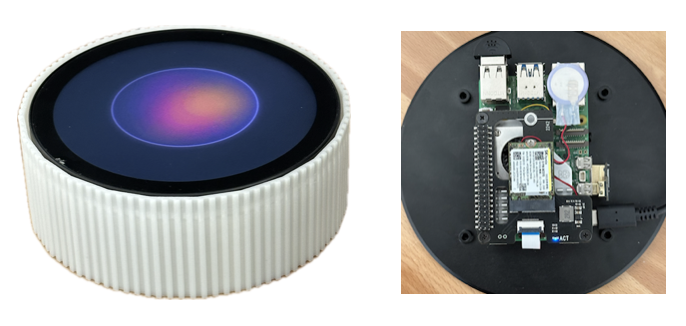
\includegraphics{device.png}}} 
	%        {x-dim}{y-dim}
	% ! means proportional scaling
	\end{center}
	\vspace{-5mm} % just to remove the extra space between the figure and the
				  % caption
	\caption{Picture of the device showcasing its compact design.}
	\label{device}
	\end{figure}

\subsection{Hardware Design}
Our project is centered around the Raspberry Pi 5, for its compact form factor and robust community support, making it ideal for prototyping intelligent devices. The main hardware features include:
\begin{itemize}
	\item \textbf{Raspberry Pi 5:} The brain of the device, that powers the user interface and manages communication with the external server for AI processing.
	\item \textbf{Touchscreen Display:} A 5-inch 1080px by 1080px round capacitive touchscreen offers a direct and intuitive interface for user interaction, allowing users to navigate the assistant's features with ease. The screen is also very sharp and bright, with a high pixel density, ensuring that all elements are displayed clearly.
	\item \textbf{Microphone:} Integrated into the device, it captures audio inputs for voice commands and queries, facilitating a hands-free user experience. 
	\item \textbf{Power Circuitry:} We utilize two 18650 Li-ion batteries to power the device, with a custom-designed power circuit layout inside the enclosure. The batteries are rechargeable via a USB-C port, ensuring that the device can be used for extended periods without needing to be plugged in. The port can also be used to power the device directly from a power source.
	\item \textbf{3D-Printed Enclosure:} Custom-designed to house the Raspberry Pi and its peripherals snugly, ensuring durability and portability while maintaining a stylish and sophisticated appearance. The enclosure is designed to be compact and lightweight, making it easy to carry around and use in various settings. It has carefully placed openings for the microphone, USB-C port, and ventilation for heat dissipation.
\end{itemize}
The combination of these components within a single device ensures that our AI assistant is not only functional but also practical for everyday use in varied environments.

\subsection{User Interface}
The user interface of our AI assistant is designed with a focus on simplicity and efficiency, leveraging PyQt5 to create a minimalist yet effective user interaction layer. PyQt5, a set of Python bindings for the Qt application framework, enables us to develop a cross-platform GUI that functions seamlessly on various operating systems, ensuring broad accessibility, and flexibility in deployment if we choose to expand the system to other platforms in the future. 
\begin{figure}[bht]
	\begin{center}
	{\resizebox{3.2in}{!}{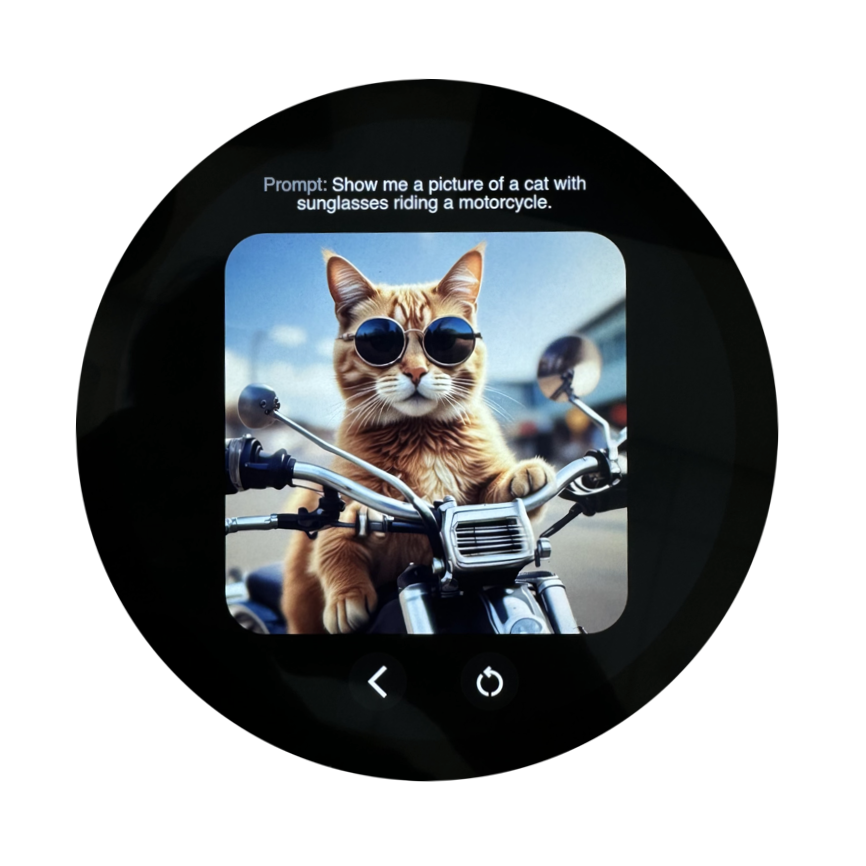
\includegraphics{ui.png}}} 
	%        {x-dim}{y-dim}
	% ! means proportional scaling
	\end{center}
	\vspace{-5mm} % just to remove the extra space between the figure and the
				  % caption
	\caption{Picture of the UI showcasing the image generation functionality.}
	\label{device}
\end{figure}

The touch screen is the primary input method for the user, allowing them to interact with the assistant through intuitive gestures and taps.
The UI is optimized for touch inputs, making it easy to navigate the interface, with large clear buttons. The UI avoids clutter by displaying only essential elements, reducing cognitive load and enhancing user experience. The interface has a home animation, then a recording screen, and finally a response screen that displays the generated response (based on its type). The only UI elements are the recording button on the home screen, and a back and regenerate button on the response screen. 
Visual feedback is provided for interactions to confirm user actions, such as pressing buttons or swiping through screens.
The interface dynamically adjusts to account for the round screen, ensuring that all elements are displayed correctly.

\subsection{Server Configuration and Operation}
Due to the Raspberry Pi 5's lack of native AI accelerators, and relatively poor performance at ML workloads, we have opted to use the Pi as a client device that is used purely for user interaction. The Pi is connected to a workstation equipped with an Intel i9-13900K CPU and an NVIDIA RTX 4090 GPU, which is used to process the AI models. 
The Pi communicates with the workstation via a Flask-based server, which is designed to manage and process user interactions. The server is configured to handle requests on port 5000, and is secured to only accept connections from Colby IP ranges (137.146.x.x), ensuring controlled accessibility and enhancing security. For every audio prompt given by the user, the Pi sends the audio data to the server as a POST request. The server then processes the audio data, transcribes it, classifies it, performs the necessary task, and sends the response back to the Pi. The Pi then displays the response to the user.

\subsection{Modular Integration of Functions}
Each functionality—audio transcription, text classification, and task-specific processing—is encapsulated within separate modules. This modular approach enhances the maintainability and scalability of the system. The server workflow is as follows:
\begin{itemize}
    \item \textbf{Transcription Module (OpenAI Whisper):} Converts audio input into textual data, also determining the language of the input. This is crucial for supporting multilingual interactions. If the input is in a language other than English, the system translates it to English for further processing, as all our models are trained on English data. It stores the source language of the input for translation back to the original language (if needed).\cite{radford2022whisper}
    \item \textbf{Classification Module (Google Gemma 7B Instruct):} Analyzes the (translated) transcribed text to determine the nature of the request (e.g., whether the request pertains to image generation, translation, or chatting). It then returns the classification to the server as a JSON object with the classification label and simplified prompt.\cite{gemmateam2024gemma}
    \item \textbf{Task-Specific Processing:} Depending on the classification outcome, the request is routed to the appropriate service:
    \begin{itemize}
		\item \textbf{Chat Interaction (Mistral 7B):} If the task involves chatting, the request is sent to the chat model. The generated response is then sent back to the Pi for display (translated back to the source language if needed), along with the original prompt (in the source language).\cite{jiang2023mistral,nllbteam2022language}
        \item \textbf{Image Generation (SDXL-Lightning):} If the task involves generating images, the request is sent to the image generation model. The generated image is then sent back to the Pi for display as a base64-encoded string, along with the original prompt (in the source language).
		\cite{lin2024sdxllightning}
        \item \textbf{Translation (Meta NLLM):} If the task involves translating text, the request is sent to the translation model. The translated text is then sent back to the Pi for display, along with the original prompt (in the source language) and the source and target languages.\cite{nllbteam2022language}
    \end{itemize}
\end{itemize}
\begin{figure}[bht]
	\begin{center}
	{\resizebox{4.9in}{!}{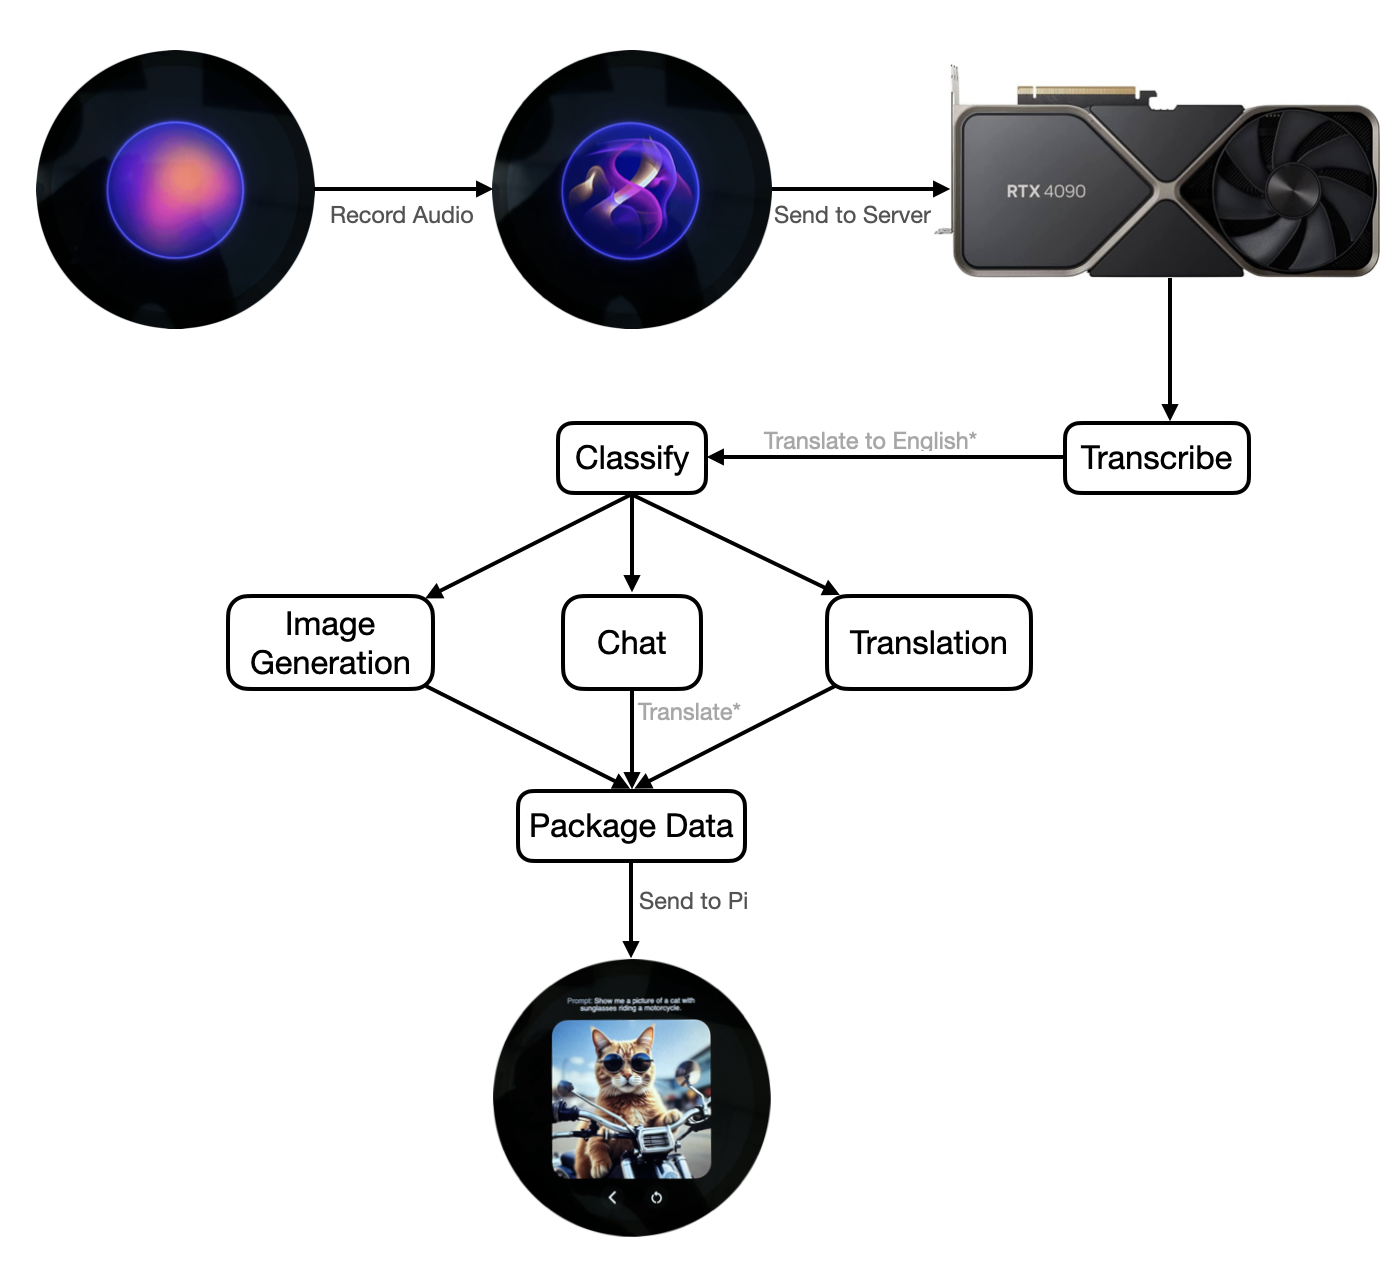
\includegraphics{chart.png}}}
	%        {x-dim}{y-dim}
	% ! means proportional scaling
	\end{center}
	\vspace{-5mm} % just to remove the extra space between the figure and the
				  % caption
\caption{Diagram illustrating the server communication workflow and task processing.}
	\label{server}
\end{figure}
This modular design allows for easy integration of new models and functionalities, ensuring that the system can be easily expanded and adapted to meet evolving user needs. Figure~\ref{server} illustrates the workflow of the server communication and task processing.

\subsection{User Security and Privacy}
The server employs stringent security measures including:
\begin{itemize}
	\item \textbf{Authentication:} Requests are authenticated using a predefined secret key, ensuring that only authorized users can interact with the system. The server ensures that all received data, particularly audio, is validated for presence and integrity before processing. 
	\item \textbf{Privacy:} The server is designed to handle all data locally, ensuring that user information is not stored or transmitted outside the system. This privacy-centric design ensures that user data remains secure and confidential. The server also does not store or log any user data, further enhancing privacy.
\end{itemize}

\subsection{Testing, Validation, and Refinement}
The assistant undergoes rigorous testing and validation across various scenarios to verify its performance on privacy, usability, accuracy, and user satisfaction. This includes stress testing the device under various environmental conditions and user testing to gather feedback on the interface's intuitiveness and responsiveness. Based on user feedback and performance data, we continuously refine our system throughout development to better meet user needs and ensure that the hardware and software components function correctly in real-world scenarios. 

\section{Results}
\subsection{User Reflection}
We conducted a user reflection survey to gather feedback on the assistant's performance. Inspired by the methodological framework in "Evaluation of Emotional Satisfaction Using Questionnaires in Voice-Based Human–AI Interaction," we broke down the survey into different factors that may affect user satisfaction. The survey was designed to evaluate aspects such as user satisfaction, privacy concerns, and suggestions for future improvements. We analyzed the correlation between various user satisfaction metrics and the assistant's performance with overall satisfaction to identify the most crucial factors affecting user satisfaction and pinpoint areas for improvement.

\begin{figure}[bht]
	\begin{center}
	{\resizebox{4.5in}{!}{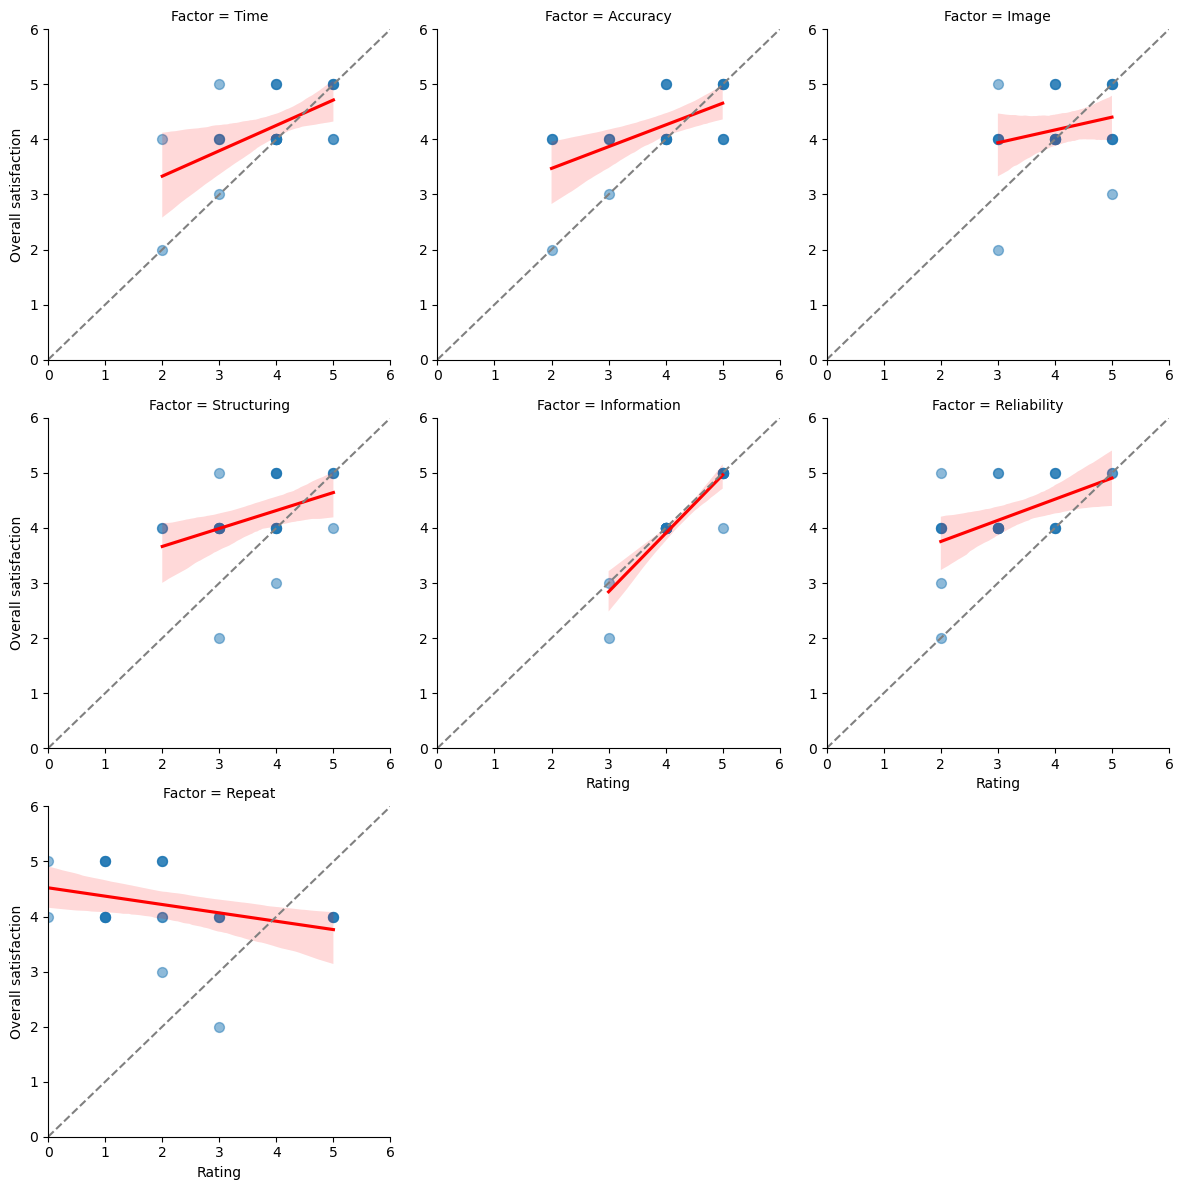
\includegraphics{dotplot.png}}}
	%        {x-dim}{y-dim}
	% ! means proportional scaling
	\end{center}
	\vspace{-5mm} % just to remove the extra space between the figure and the caption
    \caption{Dot Plot with Linear Tendency of User Satisfaction factors}
	\label{dotplot}
\end{figure}

The depth of information in the responses provided by the system had the highest positive correlation with overall user satisfaction, suggesting that users value comprehensive and detailed answers. Efficiency metrics such as the accuracy of speech recognition and the time it took for the assistant to respond were also significantly correlated with satisfaction, indicating the importance of a responsive and accurate system.
The need to repeat questions negatively affected user satisfaction, highlighting an area for immediate improvement.\\

% Figure 1: Dot Plot with Linear Tendency Line for Depth of Information and User Satisfaction.
% Figure 2: Correlation Bar Graph of User Satisfaction Metrics.
% Figure 3: Composite Graph of All Factors with Linear Regression Analysis.


\begin{figure}[bht]
	\begin{center}
	{\resizebox{4.5in}{!}{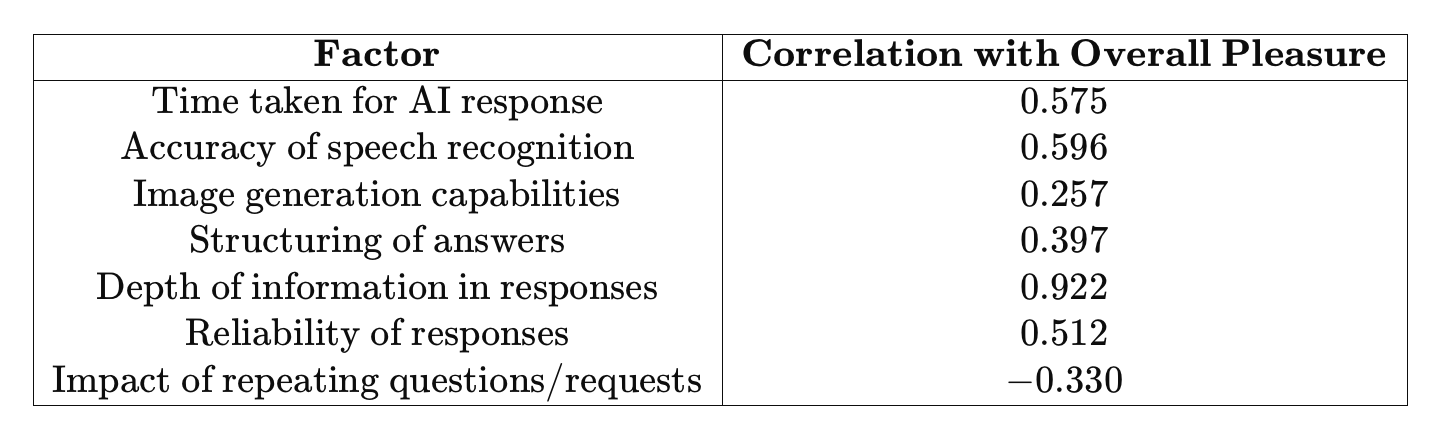
\includegraphics{factorchart.png}}}
	%        {x-dim}{y-dim}
	% ! means proportional scaling
	\end{center}
	\vspace{-5mm} % just to remove the extra space between the figure and the caption
\caption{User Satisfaction factors correlation parameters}
	\label{factorchart}
	\end{figure}
 
With the correlation calculation \eqref{correlation}, we numerically calculate the correlation parameter of each factors. The correlation analysis of user satisfaction metrics underscores the importance of the structure of a response, with a significant correlation, highlighting that users value clear and logical answers the most. Speech recognition accuracy and response time also affect satisfaction, indicating that effective communication and speed are key to a positive user experience. Other features like image generation, though beneficial, are less critical to overall satisfaction.

\subsection{Future Development}
User Experience Enhancements: Users appreciated the quick responsiveness and user-friendly interface of the assistant. Potential enhancements could include reducing distractions from background noise and updating the database more frequently to ensure the information remains current.

Feature Additions: Several suggestions for new features were mentioned, such as improved handling of multilingual interactions, more basic informational queries, and enhancements in image generation capabilities, especially concerning copyright issues. Future improvements could include fine-tuning the models, particularly the classifier, as we are currently relying on pre-trained models.

Privacy and Trust: Given the strong focus on privacy, it might be beneficial to include more explicit information or features that reassure users about how their data is being handled and protected. This could help in building trust and ensuring a more secure user experience.

These findings and user feedback will guide our development strategy as we aim to enhance user satisfaction and broaden the capabilities of our AI assistant.


\section*{Acknowledgements}
We want to thank Prof.~Ying Li for her invaluable feedback and her guidance throughout this project. \\
We would also like to thank MuleWorks for help with 3D printing the enclosure for our device.


\begin{thebibliography}{1}

\bibitem{carmody2021privacy}
Carmody, J., Shringarpure, S., and Van de Venter, G. (2021), ``\emph{AI and privacy concerns: a smart meter case study},'' Journal of Information, Communication and Ethics in Society, Vol. 19 No. 4, pp. 492--505. \href{https://doi.org/10.1108/JICES-04-2021-0042}{https://doi.org/10.1108/JICES-04-2021-0042}

\bibitem{shin2021emotional}
Shin, Jong-Gyu, Ga-Young Choi, Han-Jeong Hwang, and Sang-Ho Kim (2021), ``\emph{Evaluation of Emotional Satisfaction Using Questionnaires in Voice-Based Human-AI Interaction},'' Applied Sciences 11, no. 4: 1920. \href{https://doi.org/10.3390/app11041920}{https://doi.org/10.3390/app11041920}

\bibitem{radford2022whisper}
Radford, Alec, Kim, Jong Wook, Xu, Tao, Brockman, Greg, McLeavey, Christine, and Sutskever, Ilya (2022), ``\emph{Robust Speech Recognition via Large-Scale Weak Supervision},'' \emph{arXiv preprint} arXiv:2212.04356. \href{https://doi.org/10.48550/ARXIV.2212.04356}{https://doi.org/10.48550/ARXIV.2212.04356}

\bibitem{gemmateam2024gemma}
Gemma Team et al. (2024), ``\emph{Gemma: Open Models Based on Gemini Research and Technology},'' \emph{arXiv preprint} arXiv:2403.08295. \url{https://arxiv.org/abs/2403.08295}

\bibitem{jiang2023mistral}
Jiang, Albert Q. et al. (2023), ``\emph{Mistral 7B},'' \emph{arXiv preprint} arXiv:2310.06825. \url{https://arxiv.org/abs/2310.06825}

\bibitem{lin2024sdxllightning}
Lin, Shanchuan and Wang, Anran and Yang, Xiao (2024), ``\emph{SDXL-Lightning: Progressive Adversarial Diffusion Distillation},'' \emph{arXiv preprint} arXiv:2402.13929. \url{https://arxiv.org/abs/2402.13929}

\bibitem{nllbteam2022language}
NLLB Team et al. (2022). ``\emph{No Language Left Behind: Scaling Human-Centered Machine Translation},'' \emph{arXiv preprint} arXiv:2207.04672. \url{https://arxiv.org/abs/2207.04672}

\end{thebibliography}

\newpage 
\section*{Appendix}


  \begin{equation}\label{correlation}
   Correlation = \frac{n(\sum Factor\times Satisf) - (\sum Factor)(\sum Satisf)}{\sqrt{[n\sum Factor^2 - (\sum Factor)^2][n\sum Satisf^2 - (\sum Satisf)^2]}}
  \end{equation}




\begin{figure}[bht]
	\begin{center}
	{\resizebox{4.5in}{!}{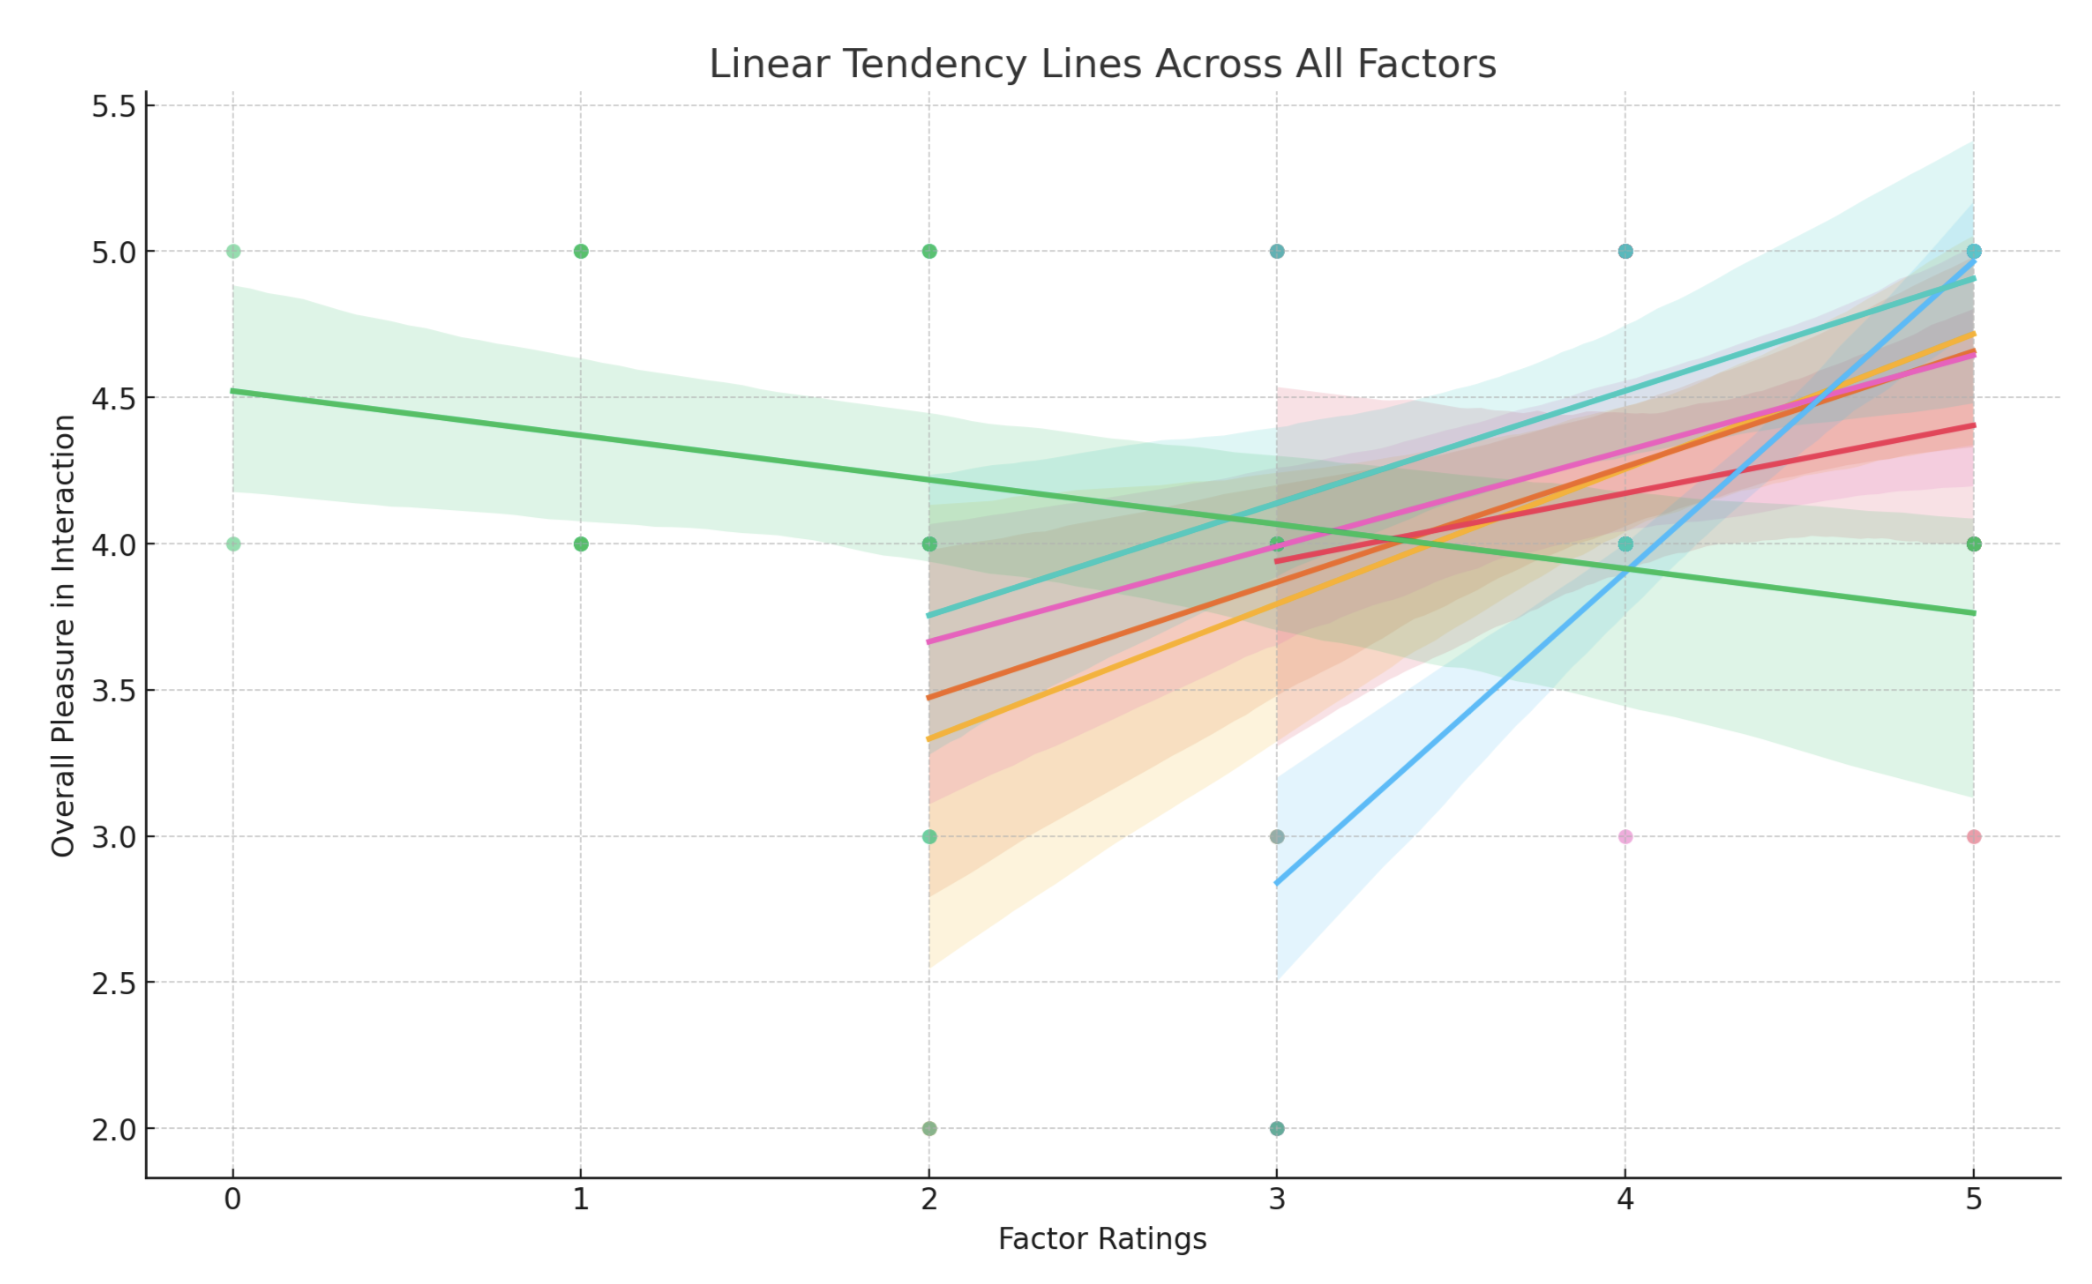
\includegraphics{linear dependency.png}}}
	%        {x-dim}{y-dim}
	% ! means proportional scaling
	\end{center}
	\vspace{-5mm} % just to remove the extra space between the figure and the caption
\caption{Linear Tendency of User Satisfaction factors}
	\label{linear tendency}
	\end{figure}


\begin{figure}[bht]
	\begin{center}
	{\resizebox{4.5in}{!}{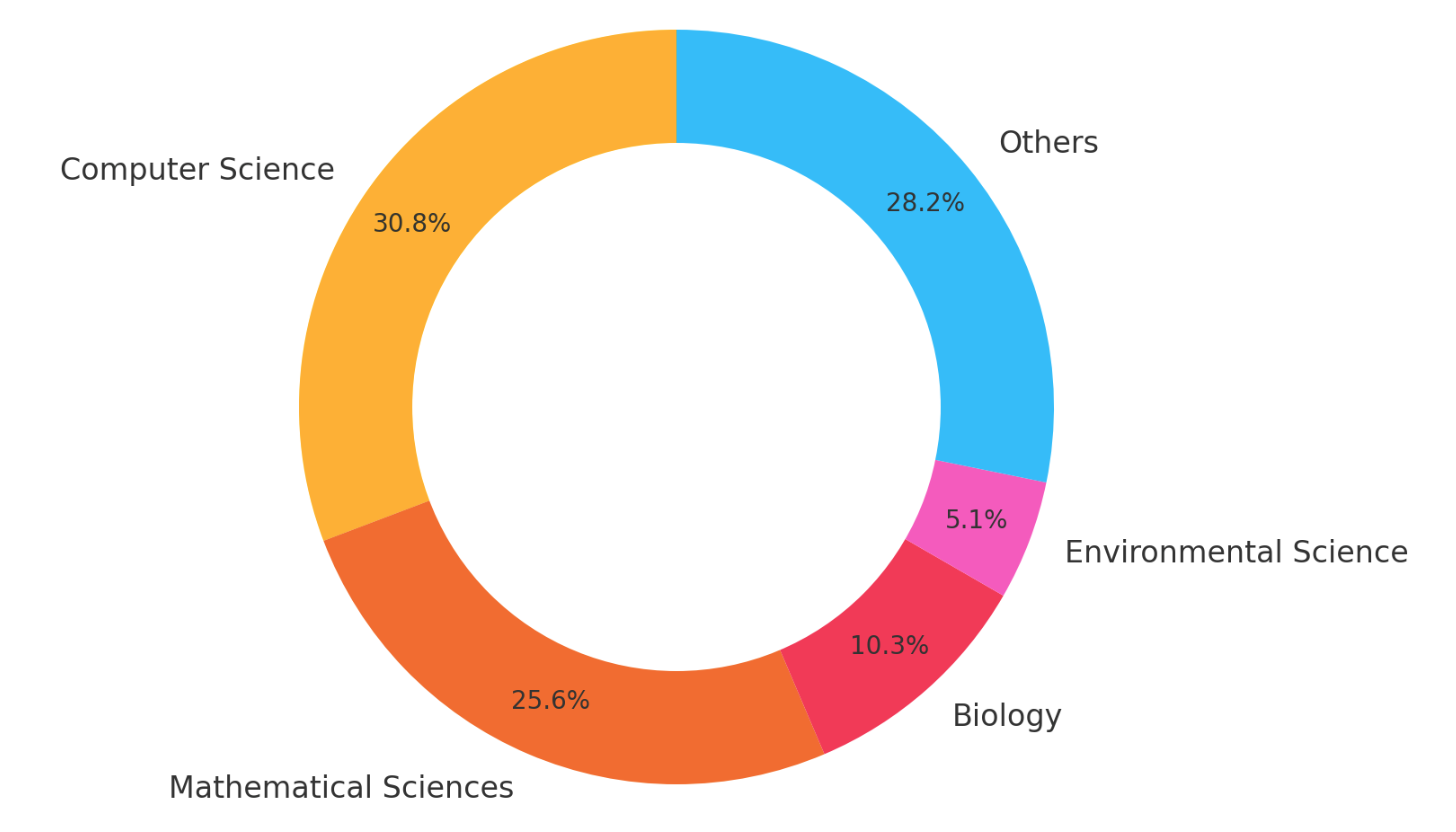
\includegraphics{majors.png}}}
	%        {x-dim}{y-dim}
	% ! means proportional scaling
	\end{center}
	\vspace{-5mm} % just to remove the extra space between the figure and the caption
\caption{Majors}
	\label{majors}
	\end{figure}










\end{document}
